\section{Theorie}
\label{sec:Theorie}


        \subsection{Magnetisches Moment des Elektrons}

            Das magnetische Moment eines Elektrons wird durch einen Drehimpuls erzeugt. 
            Im Elektron gibt es zwei Arten von Drehimpulsen, die je ihr eigenes magnetisches 
            Moment erzeugen. 
            Aus dem Bahndrehimpuls $\vec{l}$, dessen Betrag sich mithilfe der Quantenzahl 
            $l$ als $\lvert \vec{l}\rvert = \sqrt{l(l+1)}\hbar$ schreiben lässt, folgt das magnetische 
            Moment 

            \begin{align*}
                \vec{\mu}_l=-\mu_B\frac{\vec{l}}{\hbar} = -\mu_B \sqrt{l(l+1)}\vec{l}_e.
            \end{align*}

            Dieser Ausdruck enthält das Bohrsche Magneton 

            \begin{align*}
                \mu_B = -\frac12 e_0 \frac\hbar m_0.
            \end{align*}

            Aus dem Spin $\vec{s}$ mit Betrag $\lvert \vec{s}\rvert = \sqrt{s(s+1)}\hbar$ ergibt 
            sich das magnetische Moment

            \begin{align*}
                \vec{\mu}_s = -\symup{g}_s \frac{\mu_B}\hbar \vec{s}.
            \end{align*}

            Dies unterscheidet sich in seiner Struktur vom magnetischen Moment des Bahndrehimpulses 
            durch den Land\'{e}faktor $\symup{g}_s\approx 2$ des Elektrons.

        \subsection{Kopplungen der Drehimpulse und magnetischen Momente mehrerer Elektronen}

            Je nach Kernladungszahl des Atoms koppeln die einzelnen magnetischen Momente 
            und Drehimpulse unterschiedlich aneinander. Für die beiden Grenzfälle sehr leichter 
            und sehr schwerer Atome lassen sich eindeutige Regeln ableiten. Mittelschwere Atome 
            werden von beiden Grenzfällen beeinflusst. 

            \subsubsection{LS-Kopplung}

                Die LS-Kopplung spielt eine wichtige Rolle bei kleinen Kernladungszahlen. 
                Dabei wechselwirken die Bahndrehimpulse bzw. die Spins verschiedener Elektronen 
                untereinander so stark, dass sie zum Gesamtbahndrehimpuls bzw. Gesamtspin 
                aufsummiert werden können: 

                \begin{align*}
                    \vec{L} &= \sum \vec{l}_i\\
                    \vec{S} &= \sum \vec{s}_i.
                \end{align*}


                Für die Beträge der Summen gilt analog zu den Einzelbeträgen

                \begin{align*}
                    \lvert\vec{L}\rvert &= \sqrt{L(L+1)}\hbar\\ 
                    \lvert\vec{S}\rvert &= \sqrt{S(S+1)}\hbar.
                \end{align*}

                $L$ kann 0, 1, 2 oder 3 sein. Aus $S$ wird die Multiplizität $M=2S+1$ errechnet.
                Ebenfalls lässt sich dem Gesamtbahndrehimpuls und dem Gesamtspin je ein 
                magnetisches Moment der Form

                \begin{align*}
                    \lvert\vec{\mu}_L\rvert &= \mu_B\sqrt{L(L+1)}\\
                    \lvert\vec{\mu}_S\rvert &= \symup{g}_s\mu_B\sqrt{S(S+1)}\\
                \end{align*}

                zuordnen.
                In kleinen Magnetfeldern wird bei der LS-Kopplung der Gesamtdrehimpuls 

                \begin{align*}
                    \vec{J}=\vec{L}+\vec{S}
                \end{align*}

                gebildet. Er hat den Betrag 

                \begin{align*}
                    \lvert \vec{J}\rvert = \sqrt{J(J+1)}\hbar.
                \end{align*}                

            \subsubsection{jj-Kopplung}

                Im Fall sehr schwerer Atome überwiegt die Wechselwirkung zwischen Bahndrehimpuls 
                und Spin innerhalb eines Elektrons. Deshalb werden für alle Elektronen 
                Gesamtdrehimpulse gebildet, die anschließend addiert werden können:

                \begin{align*}
                    \vec{j}_i = \vec{l}_i+\vec{s}_i \Rightarrow \vec{J} = \sum \vec{j}_i.
                \end{align*}

        \subsection{Energieniveaus im Magnetfeld}

            \subsubsection{Aufspaltung der Energie durch ein Magnetfeld}

                Das magnetische Moment durch den Drehimpuls $\vec{J}$ 
                wird durch die Gleichungen 

                \begin{align*}
                    \vec{\mu}_J &= \vec{\mu}_L+\vec{\mu}_S\\
                    \lvert \vec{\mu}_J\rvert &= \mu_B\symup{g}_J\sqrt{J(J+1)}
                \end{align*}

                definiert.
                Der Land\'{e}faktor ist dabei durch 

                \begin{align*}
                    \symup{g}_J = \frac{3J(J+1)+S(S+1)-L(L+1)}{2J(J+1)}
                \end{align*}

                gegeben.
                Für die z-Komponente des Drehimpulses gibt es im Magnetfeld $2J+1$ 
                Einstellmöglichkeiten. Dies führt zu einer Aufspaltung in Energieniveaus 
                mit 

                \begin{align*}
                    E = E_0 + m\symup{g}_J\mu_B B\,\,\,\,\text{mit}\,\,-J\leq m\leq J.
                \end{align*}


            \subsubsection{Auswahlregeln}

                Zwischen Energieniveaus, die zu unterschiedlichen Gesamtdrehimpulsen 
                gehören, sind nicht alle Übergänge erlaubt. Die sogenannten Auswahlregeln
                besagen, dass Übergänge nur stattfinden können, wenn die Differenz 
                der zu den Niveaus gehörenden $m$ $\pm1$ oder 0 beträgt.
                Für den Übergang mit Differenz 0 ist die emittierte Spektrallinie ($\pi$)
                linear in Richtung des Magnetfeldes polarisiert. Bei den anderen beiden 
                Übergängen liegt entgegengesetztes zirkular polarisiertes Licht vor. 
                Die Polarisation der $\sigma-$Linien ist senkrecht zum Feld.


        \subsection{Zeeman-Effekt}

            Der Zeeman-Effekt beschreibt das Phänomen, dass sich die Anzahl von 
            Spektrallinien vergrößert, wenn an die Lichtquelle ein Magnetfeld angelegt wird.
            Anhand der Größe des Gesamtspins kann zwischen normalem und anormalem Zeeman-Effekt 
            unterschieden werden.

            \subsubsection{Normaler Zeeman-Effekt}

                Beim normalen Zeeman-Effekt beträgt der Gesamtspin der Elektronenhülle 0. 
                Dies hat zur Folge, dass der Gesamtbahndrehimpuls gleich dem Gesamtdrehimpuls ist.
                Für den Land\'{e}faktor folgt somit, dass er unabhängig vom 
                vorliegenden $J$ immer 1 ist. Beim normalen Zeeman-Effekt spaltet sich eine 
                Spektrallinie durch das Magnetfeld in 3 einzelne auf. 
                In Abb. \ref{fig:rot} ist die Aufspaltung der roten Cadmium-Linie zu sehen, 
                welche durch den Übergang von dem Niveau $J_2$ zum Niveau $J_1$ erzeugt wird.

                \begin{figure}
                    \centering
                    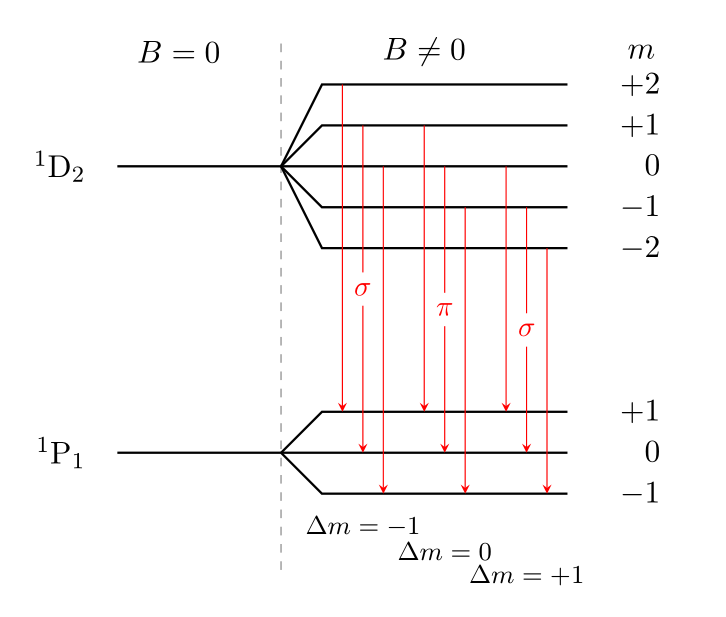
\includegraphics[height=7cm]{rot.png}
                    \caption{Darstellung der Aufspaltung der roten Cadmium-Linie, welche beim Übergang 
                    $^{1}\symup{P}_1 \to$\,$^{1}\symup{D}_2$ entsteht. Zu erkennen sind die drei Liniengruppen, welche 
                    je eine Spektrallinie verursachen. Davon sind zwei $\sigma-$polarisiert und die dritte ist $\pi-$polarisiert \cite{josh}.}
                    \label{fig:rot}
                \end{figure}

                Durch Anschalten des Magnetfelds spalten sich die Linien mit Energie $E$ 
                in $2J+1$ Unterlinien auf, deren Energieniveaus bei $E+m\mu_B B$ liegen. 
                Übergänge sind laut den Auswahlregeln aber nur für $\Delta m = \pm 1, 0$ erlaubt. 
                Deshalb entsteht für jedes erlaubte $\Delta m$ eine Dreiergruppe von erlaubten
                Übergängen zwischen den Unterschiedlichen $J$. 
                Da die Übergänge innerhalb einer Gruppe den gleichen Energieabstand überwinden, 
                bilden sie eine einzige Spektrallinie.


            \subsubsection{Anormaler Zeeman-Effekt}

               Beim anormalen Zeeman-Effekt ist der Spin nicht 0, sodass der Land\'{e}-Faktor für jedes 
               $J$ einzeln berechnet werden muss. Dadurch kann nicht angenommen werden, dass 
               innerhalb einer Übergangsgruppe die Energiedifferenzen gleich sind, sodass mehr Spektrallinien 
               auftreten als beim normalen Zeeman-Effekt. Beim anormalen Zeeman-Effekt werden 
               Energieniveaus der Energie $E$ aufgespalten in $E+m\symup{g}_J\mu_B B$.
               In Abb. \ref{fig:blau} ist der anormale Zeeman-Effekt 
               für die blaue Cadmium-Linie zu sehen. 
               
                \begin{figure}
                    \centering
                    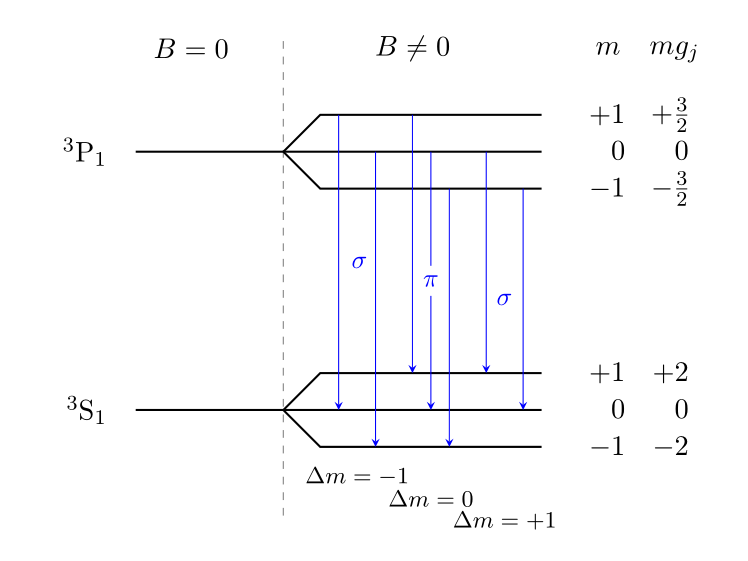
\includegraphics[height=7cm]{blau.png}
                    \caption{Darstellung der Aufspaltung der blauen Cadmium-Linie, welche beim Übergang 
                    $^{3}\symup{P}_1 \to$\,\,$^{3}\symup{S}_1$ entsteht. Zu erkennen sind grundsätzlich 7 Übergänge,
                    die verschiedene Übergangsenergien besitzen. Da der Übergang vom $m=0$ zu $m=0$ jedoch verboten ist, folgen 
                    6 Spektrallinien, wovon zwei $\pi-$ und vier $\sigma-$polarisiert sind \cite{josh}.}
                    \label{fig:blau}
                \end{figure}
               
               Für die Übergänge mit $\Delta m = \pm 1$ gibt es je 
               zwei Übergänge mit unterschiedlicher Energie, sodass daraus insgesamt 4 Spektrallinien entstehen. 
               Da der Übergang von $m=0$ zu $m=0$ verboten ist, gibt es auch für den Übergang mit
               $\Delta m  = 0$ zwei unterschiedlich energetische Übergänge, die zu insgesamt zwei 
               Spektrallinien führen. 
